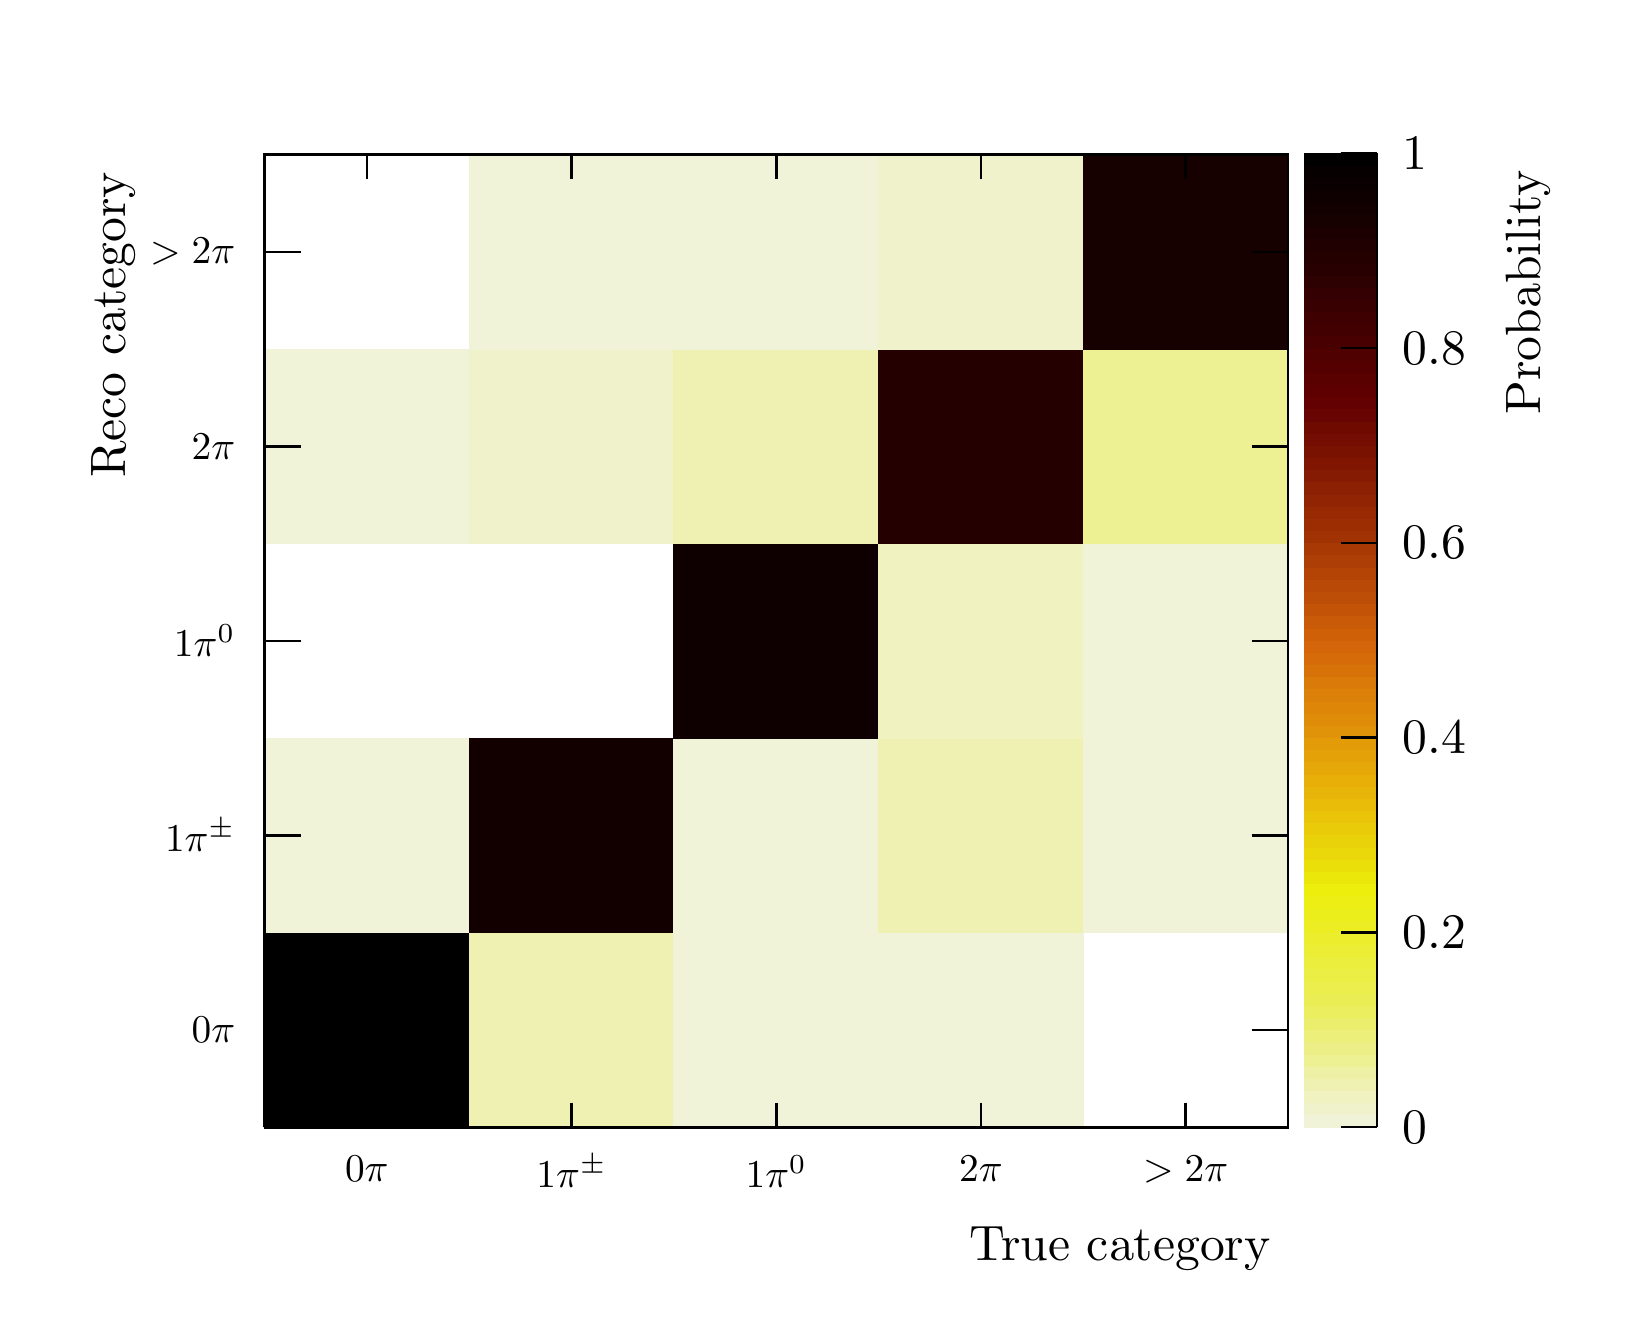
\begin{tikzpicture}
\pgfdeclareplotmark{cross} {
\pgfpathmoveto{\pgfpoint{-0.3\pgfplotmarksize}{\pgfplotmarksize}}
\pgfpathlineto{\pgfpoint{+0.3\pgfplotmarksize}{\pgfplotmarksize}}
\pgfpathlineto{\pgfpoint{+0.3\pgfplotmarksize}{0.3\pgfplotmarksize}}
\pgfpathlineto{\pgfpoint{+1\pgfplotmarksize}{0.3\pgfplotmarksize}}
\pgfpathlineto{\pgfpoint{+1\pgfplotmarksize}{-0.3\pgfplotmarksize}}
\pgfpathlineto{\pgfpoint{+0.3\pgfplotmarksize}{-0.3\pgfplotmarksize}}
\pgfpathlineto{\pgfpoint{+0.3\pgfplotmarksize}{-1.\pgfplotmarksize}}
\pgfpathlineto{\pgfpoint{-0.3\pgfplotmarksize}{-1.\pgfplotmarksize}}
\pgfpathlineto{\pgfpoint{-0.3\pgfplotmarksize}{-0.3\pgfplotmarksize}}
\pgfpathlineto{\pgfpoint{-1.\pgfplotmarksize}{-0.3\pgfplotmarksize}}
\pgfpathlineto{\pgfpoint{-1.\pgfplotmarksize}{0.3\pgfplotmarksize}}
\pgfpathlineto{\pgfpoint{-0.3\pgfplotmarksize}{0.3\pgfplotmarksize}}
\pgfpathclose
\pgfusepathqstroke
}
\pgfdeclareplotmark{cross*} {
\pgfpathmoveto{\pgfpoint{-0.3\pgfplotmarksize}{\pgfplotmarksize}}
\pgfpathlineto{\pgfpoint{+0.3\pgfplotmarksize}{\pgfplotmarksize}}
\pgfpathlineto{\pgfpoint{+0.3\pgfplotmarksize}{0.3\pgfplotmarksize}}
\pgfpathlineto{\pgfpoint{+1\pgfplotmarksize}{0.3\pgfplotmarksize}}
\pgfpathlineto{\pgfpoint{+1\pgfplotmarksize}{-0.3\pgfplotmarksize}}
\pgfpathlineto{\pgfpoint{+0.3\pgfplotmarksize}{-0.3\pgfplotmarksize}}
\pgfpathlineto{\pgfpoint{+0.3\pgfplotmarksize}{-1.\pgfplotmarksize}}
\pgfpathlineto{\pgfpoint{-0.3\pgfplotmarksize}{-1.\pgfplotmarksize}}
\pgfpathlineto{\pgfpoint{-0.3\pgfplotmarksize}{-0.3\pgfplotmarksize}}
\pgfpathlineto{\pgfpoint{-1.\pgfplotmarksize}{-0.3\pgfplotmarksize}}
\pgfpathlineto{\pgfpoint{-1.\pgfplotmarksize}{0.3\pgfplotmarksize}}
\pgfpathlineto{\pgfpoint{-0.3\pgfplotmarksize}{0.3\pgfplotmarksize}}
\pgfpathclose
\pgfusepathqfillstroke
}
\pgfdeclareplotmark{newstar} {
\pgfpathmoveto{\pgfqpoint{0pt}{\pgfplotmarksize}}
\pgfpathlineto{\pgfqpointpolar{44}{0.5\pgfplotmarksize}}
\pgfpathlineto{\pgfqpointpolar{18}{\pgfplotmarksize}}
\pgfpathlineto{\pgfqpointpolar{-20}{0.5\pgfplotmarksize}}
\pgfpathlineto{\pgfqpointpolar{-54}{\pgfplotmarksize}}
\pgfpathlineto{\pgfqpointpolar{-90}{0.5\pgfplotmarksize}}
\pgfpathlineto{\pgfqpointpolar{234}{\pgfplotmarksize}}
\pgfpathlineto{\pgfqpointpolar{198}{0.5\pgfplotmarksize}}
\pgfpathlineto{\pgfqpointpolar{162}{\pgfplotmarksize}}
\pgfpathlineto{\pgfqpointpolar{134}{0.5\pgfplotmarksize}}
\pgfpathclose
\pgfusepathqstroke
}
\pgfdeclareplotmark{newstar*} {
\pgfpathmoveto{\pgfqpoint{0pt}{\pgfplotmarksize}}
\pgfpathlineto{\pgfqpointpolar{44}{0.5\pgfplotmarksize}}
\pgfpathlineto{\pgfqpointpolar{18}{\pgfplotmarksize}}
\pgfpathlineto{\pgfqpointpolar{-20}{0.5\pgfplotmarksize}}
\pgfpathlineto{\pgfqpointpolar{-54}{\pgfplotmarksize}}
\pgfpathlineto{\pgfqpointpolar{-90}{0.5\pgfplotmarksize}}
\pgfpathlineto{\pgfqpointpolar{234}{\pgfplotmarksize}}
\pgfpathlineto{\pgfqpointpolar{198}{0.5\pgfplotmarksize}}
\pgfpathlineto{\pgfqpointpolar{162}{\pgfplotmarksize}}
\pgfpathlineto{\pgfqpointpolar{134}{0.5\pgfplotmarksize}}
\pgfpathclose
\pgfusepathqfillstroke
}
\definecolor{c}{rgb}{1,1,1};
\draw [color=c, fill=c] (0,0) rectangle (20,16.0446);
\draw [color=c, fill=c] (3,2.08579) rectangle (16,14.4401);
\definecolor{c}{rgb}{0,0,0};
\draw [c,line width=0.9] (3,2.08579) -- (3,14.4401) -- (16,14.4401) -- (16,2.08579) -- (3,2.08579);
\definecolor{c}{rgb}{1,1,1};
\draw [color=c, fill=c] (3,2.08579) rectangle (16,14.4401);
\definecolor{c}{rgb}{0,0,0};
\draw [c,line width=0.9] (3,2.08579) -- (3,14.4401) -- (16,14.4401) -- (16,2.08579) -- (3,2.08579);
\definecolor{c}{rgb}{0.00551471,0,0.000122549};
\draw [color=c, fill=c] (3,2.08579) rectangle (5.6,4.55666);
\definecolor{c}{rgb}{0.936875,0.945351,0.697027};
\draw [color=c, fill=c] (5.6,2.08579) rectangle (8.2,4.55666);
\definecolor{c}{rgb}{0.945984,0.951044,0.850727};
\draw [color=c, fill=c] (8.2,2.08579) rectangle (10.8,4.55666);
\draw [color=c, fill=c] (10.8,2.08579) rectangle (13.4,4.55666);
\draw [color=c, fill=c] (3,4.55666) rectangle (5.6,7.02752);
\definecolor{c}{rgb}{0.0716912,0,0.00159314};
\draw [color=c, fill=c] (5.6,4.55666) rectangle (8.2,7.02752);
\definecolor{c}{rgb}{0.945984,0.951044,0.850727};
\draw [color=c, fill=c] (8.2,4.55666) rectangle (10.8,7.02752);
\definecolor{c}{rgb}{0.936875,0.945351,0.697027};
\draw [color=c, fill=c] (10.8,4.55666) rectangle (13.4,7.02752);
\definecolor{c}{rgb}{0.945984,0.951044,0.850727};
\draw [color=c, fill=c] (13.4,4.55666) rectangle (16,7.02752);
\definecolor{c}{rgb}{0.0551471,0,0.00122549};
\draw [color=c, fill=c] (8.2,7.02752) rectangle (10.8,9.49838);
\definecolor{c}{rgb}{0.939911,0.947249,0.748261};
\draw [color=c, fill=c] (10.8,7.02752) rectangle (13.4,9.49838);
\definecolor{c}{rgb}{0.945984,0.951044,0.850727};
\draw [color=c, fill=c] (13.4,7.02752) rectangle (16,9.49838);
\draw [color=c, fill=c] (3,9.49838) rectangle (5.6,11.9692);
\definecolor{c}{rgb}{0.942948,0.949146,0.799494};
\draw [color=c, fill=c] (5.6,9.49838) rectangle (8.2,11.9692);
\definecolor{c}{rgb}{0.936875,0.945351,0.697027};
\draw [color=c, fill=c] (8.2,9.49838) rectangle (10.8,11.9692);
\definecolor{c}{rgb}{0.143382,0,0.00318627};
\draw [color=c, fill=c] (10.8,9.49838) rectangle (13.4,11.9692);
\definecolor{c}{rgb}{0.929791,0.940923,0.577483};
\draw [color=c, fill=c] (13.4,9.49838) rectangle (16,11.9692);
\definecolor{c}{rgb}{0.945984,0.951044,0.850727};
\draw [color=c, fill=c] (5.6,11.9692) rectangle (8.2,14.4401);
\draw [color=c, fill=c] (8.2,11.9692) rectangle (10.8,14.4401);
\definecolor{c}{rgb}{0.942948,0.949146,0.799494};
\draw [color=c, fill=c] (10.8,11.9692) rectangle (13.4,14.4401);
\definecolor{c}{rgb}{0.0882353,0,0.00196078};
\draw [color=c, fill=c] (13.4,11.9692) rectangle (16,14.4401);
\definecolor{c}{rgb}{0,0,0};
\draw [c,line width=0.9] (3,2.08579) -- (16,2.08579);
\draw [anchor=north] (4.3,1.90048) node[scale=1.42291, color=c, rotate=0]{$0\pi$};
\draw [anchor=north] (6.9,1.90048) node[scale=1.42291, color=c, rotate=0]{$1\pi^{\pm}$};
\draw [anchor=north] (9.5,1.90048) node[scale=1.42291, color=c, rotate=0]{$1\pi^{0}$};
\draw [anchor=north] (12.1,1.90048) node[scale=1.42291, color=c, rotate=0]{$2\pi$};
\draw [anchor=north] (14.7,1.90048) node[scale=1.42291, color=c, rotate=0]{$>2\pi$};
\draw [c,line width=0.9] (4.3,2.39866) -- (4.3,2.08579);
\draw [c,line width=0.9] (6.9,2.39866) -- (6.9,2.08579);
\draw [c,line width=0.9] (9.5,2.39866) -- (9.5,2.08579);
\draw [c,line width=0.9] (12.1,2.39866) -- (12.1,2.08579);
\draw [c,line width=0.9] (14.7,2.39866) -- (14.7,2.08579);
\draw [c,line width=0.9] (4.3,2.39866) -- (4.3,2.08579);
\draw [c,line width=0.9] (14.7,2.39866) -- (14.7,2.08579);
\draw [anchor= east] (16,0.545515) node[scale=1.7941, color=c, rotate=0]{ True category};
\draw [c,line width=0.9] (3,14.4401) -- (16,14.4401);
\draw [c,line width=0.9] (4.3,14.1272) -- (4.3,14.4401);
\draw [c,line width=0.9] (6.9,14.1272) -- (6.9,14.4401);
\draw [c,line width=0.9] (9.5,14.1272) -- (9.5,14.4401);
\draw [c,line width=0.9] (12.1,14.1272) -- (12.1,14.4401);
\draw [c,line width=0.9] (14.7,14.1272) -- (14.7,14.4401);
\draw [c,line width=0.9] (4.3,14.1272) -- (4.3,14.4401);
\draw [c,line width=0.9] (14.7,14.1272) -- (14.7,14.4401);
\draw [c,line width=0.9] (3,2.08579) -- (3,14.4401);
\draw [anchor= east] (2.805,3.32123) node[scale=1.42291, color=c, rotate=0]{$0\pi$};
\draw [anchor= east] (2.805,5.79209) node[scale=1.42291, color=c, rotate=0]{$1\pi^{\pm}$};
\draw [anchor= east] (2.805,8.26295) node[scale=1.42291, color=c, rotate=0]{$1\pi^{0}$};
\draw [anchor= east] (2.805,10.7338) node[scale=1.42291, color=c, rotate=0]{$2\pi$};
\draw [anchor= east] (2.805,13.2047) node[scale=1.42291, color=c, rotate=0]{$>2\pi$};
\draw [c,line width=0.9] (3.462,3.32123) -- (3,3.32123);
\draw [c,line width=0.9] (3.462,5.79209) -- (3,5.79209);
\draw [c,line width=0.9] (3.462,8.26295) -- (3,8.26295);
\draw [c,line width=0.9] (3.462,10.7338) -- (3,10.7338);
\draw [c,line width=0.9] (3.462,13.2047) -- (3,13.2047);
\draw [c,line width=0.9] (3.462,3.32123) -- (3,3.32123);
\draw [c,line width=0.9] (3.462,13.2047) -- (3,13.2047);
\draw [anchor= east] (1.08,14.4401) node[scale=1.7941, color=c, rotate=90]{ Reco category};
\draw [c,line width=0.9] (16,2.08579) -- (16,14.4401);
\draw [c,line width=0.9] (15.538,3.32123) -- (16,3.32123);
\draw [c,line width=0.9] (15.538,5.79209) -- (16,5.79209);
\draw [c,line width=0.9] (15.538,8.26295) -- (16,8.26295);
\draw [c,line width=0.9] (15.538,10.7338) -- (16,10.7338);
\draw [c,line width=0.9] (15.538,13.2047) -- (16,13.2047);
\draw [c,line width=0.9] (15.538,3.32123) -- (16,3.32123);
\draw [c,line width=0.9] (15.538,13.2047) -- (16,13.2047);
\definecolor{c}{rgb}{0.945984,0.951044,0.850727};
\draw [color=c, fill=c] (16.2117,2.08914) rectangle (17.1309,2.24373);
\definecolor{c}{rgb}{0.942948,0.949146,0.799494};
\draw [color=c, fill=c] (16.2117,2.24373) rectangle (17.1309,2.39833);
\definecolor{c}{rgb}{0.939911,0.947249,0.748261};
\draw [color=c, fill=c] (16.2117,2.39833) rectangle (17.1309,2.55292);
\definecolor{c}{rgb}{0.936875,0.945351,0.697027};
\draw [color=c, fill=c] (16.2117,2.55292) rectangle (17.1309,2.70752);
\definecolor{c}{rgb}{0.933839,0.943453,0.645794};
\draw [color=c, fill=c] (16.2117,2.70752) rectangle (17.1309,2.86212);
\definecolor{c}{rgb}{0.929791,0.940923,0.577483};
\draw [color=c, fill=c] (16.2117,2.86212) rectangle (17.1309,3.01671);
\definecolor{c}{rgb}{0.926755,0.939026,0.526249};
\draw [color=c, fill=c] (16.2117,3.01671) rectangle (17.1309,3.17131);
\definecolor{c}{rgb}{0.923719,0.937128,0.475016};
\draw [color=c, fill=c] (16.2117,3.17131) rectangle (17.1309,3.32591);
\definecolor{c}{rgb}{0.920683,0.935231,0.423782};
\draw [color=c, fill=c] (16.2117,3.32591) rectangle (17.1309,3.4805);
\definecolor{c}{rgb}{0.917647,0.933333,0.372549};
\draw [color=c, fill=c] (16.2117,3.4805) rectangle (17.1309,3.6351);
\definecolor{c}{rgb}{0.919118,0.933333,0.331373};
\draw [color=c, fill=c] (16.2117,3.6351) rectangle (17.1309,3.78969);
\definecolor{c}{rgb}{0.920221,0.933333,0.30049};
\draw [color=c, fill=c] (16.2117,3.78969) rectangle (17.1309,3.94429);
\definecolor{c}{rgb}{0.921324,0.933333,0.269608};
\draw [color=c, fill=c] (16.2117,3.94429) rectangle (17.1309,4.09889);
\definecolor{c}{rgb}{0.922426,0.933333,0.238725};
\draw [color=c, fill=c] (16.2117,4.09889) rectangle (17.1309,4.25348);
\definecolor{c}{rgb}{0.923529,0.933333,0.207843};
\draw [color=c, fill=c] (16.2117,4.25348) rectangle (17.1309,4.40808);
\definecolor{c}{rgb}{0.924632,0.933333,0.176961};
\draw [color=c, fill=c] (16.2117,4.40808) rectangle (17.1309,4.56267);
\definecolor{c}{rgb}{0.926103,0.933333,0.135784};
\draw [color=c, fill=c] (16.2117,4.56267) rectangle (17.1309,4.71727);
\definecolor{c}{rgb}{0.927206,0.933333,0.104902};
\draw [color=c, fill=c] (16.2117,4.71727) rectangle (17.1309,4.87187);
\definecolor{c}{rgb}{0.928309,0.933333,0.0740196};
\draw [color=c, fill=c] (16.2117,4.87187) rectangle (17.1309,5.02646);
\definecolor{c}{rgb}{0.929412,0.933333,0.0431373};
\draw [color=c, fill=c] (16.2117,5.02646) rectangle (17.1309,5.18106);
\definecolor{c}{rgb}{0.926838,0.907598,0.0420343};
\draw [color=c, fill=c] (16.2117,5.18106) rectangle (17.1309,5.33565);
\definecolor{c}{rgb}{0.923407,0.873284,0.0405637};
\draw [color=c, fill=c] (16.2117,5.33565) rectangle (17.1309,5.49025);
\definecolor{c}{rgb}{0.920833,0.847549,0.0394608};
\draw [color=c, fill=c] (16.2117,5.49025) rectangle (17.1309,5.64485);
\definecolor{c}{rgb}{0.91826,0.821814,0.0383578};
\draw [color=c, fill=c] (16.2117,5.64485) rectangle (17.1309,5.79944);
\definecolor{c}{rgb}{0.915686,0.796078,0.0372549};
\draw [color=c, fill=c] (16.2117,5.79944) rectangle (17.1309,5.95404);
\definecolor{c}{rgb}{0.913113,0.770343,0.036152};
\draw [color=c, fill=c] (16.2117,5.95404) rectangle (17.1309,6.10864);
\definecolor{c}{rgb}{0.909681,0.736029,0.0346814};
\draw [color=c, fill=c] (16.2117,6.10864) rectangle (17.1309,6.26323);
\definecolor{c}{rgb}{0.907108,0.710294,0.0335784};
\draw [color=c, fill=c] (16.2117,6.26323) rectangle (17.1309,6.41783);
\definecolor{c}{rgb}{0.904534,0.684559,0.0324755};
\draw [color=c, fill=c] (16.2117,6.41783) rectangle (17.1309,6.57242);
\definecolor{c}{rgb}{0.901961,0.658824,0.0313726};
\draw [color=c, fill=c] (16.2117,6.57242) rectangle (17.1309,6.72702);
\definecolor{c}{rgb}{0.895343,0.634191,0.0317402};
\draw [color=c, fill=c] (16.2117,6.72702) rectangle (17.1309,6.88162);
\definecolor{c}{rgb}{0.888726,0.609559,0.0321078};
\draw [color=c, fill=c] (16.2117,6.88162) rectangle (17.1309,7.03621);
\definecolor{c}{rgb}{0.879902,0.576716,0.032598};
\draw [color=c, fill=c] (16.2117,7.03621) rectangle (17.1309,7.19081);
\definecolor{c}{rgb}{0.873284,0.552083,0.0329657};
\draw [color=c, fill=c] (16.2117,7.19081) rectangle (17.1309,7.3454);
\definecolor{c}{rgb}{0.866667,0.527451,0.0333333};
\draw [color=c, fill=c] (16.2117,7.3454) rectangle (17.1309,7.5);
\definecolor{c}{rgb}{0.860049,0.502819,0.033701};
\draw [color=c, fill=c] (16.2117,7.5) rectangle (17.1309,7.6546);
\definecolor{c}{rgb}{0.853431,0.478186,0.0340686};
\draw [color=c, fill=c] (16.2117,7.6546) rectangle (17.1309,7.80919);
\definecolor{c}{rgb}{0.844608,0.445343,0.0345588};
\draw [color=c, fill=c] (16.2117,7.80919) rectangle (17.1309,7.96379);
\definecolor{c}{rgb}{0.83799,0.420711,0.0349265};
\draw [color=c, fill=c] (16.2117,7.96379) rectangle (17.1309,8.11838);
\definecolor{c}{rgb}{0.831373,0.396078,0.0352941};
\draw [color=c, fill=c] (16.2117,8.11838) rectangle (17.1309,8.27298);
\definecolor{c}{rgb}{0.810784,0.37549,0.0330882};
\draw [color=c, fill=c] (16.2117,8.27298) rectangle (17.1309,8.42758);
\definecolor{c}{rgb}{0.790196,0.354902,0.0308824};
\draw [color=c, fill=c] (16.2117,8.42758) rectangle (17.1309,8.58217);
\definecolor{c}{rgb}{0.762745,0.327451,0.0279412};
\draw [color=c, fill=c] (16.2117,8.58217) rectangle (17.1309,8.73677);
\definecolor{c}{rgb}{0.742157,0.306863,0.0257353};
\draw [color=c, fill=c] (16.2117,8.73677) rectangle (17.1309,8.89137);
\definecolor{c}{rgb}{0.721569,0.286275,0.0235294};
\draw [color=c, fill=c] (16.2117,8.89137) rectangle (17.1309,9.04596);
\definecolor{c}{rgb}{0.70098,0.265686,0.0213235};
\draw [color=c, fill=c] (16.2117,9.04596) rectangle (17.1309,9.20056);
\definecolor{c}{rgb}{0.680392,0.245098,0.0191176};
\draw [color=c, fill=c] (16.2117,9.20056) rectangle (17.1309,9.35515);
\definecolor{c}{rgb}{0.659804,0.22451,0.0169118};
\draw [color=c, fill=c] (16.2117,9.35515) rectangle (17.1309,9.50975);
\definecolor{c}{rgb}{0.632353,0.197059,0.0139706};
\draw [color=c, fill=c] (16.2117,9.50975) rectangle (17.1309,9.66435);
\definecolor{c}{rgb}{0.611765,0.176471,0.0117647};
\draw [color=c, fill=c] (16.2117,9.66435) rectangle (17.1309,9.81894);
\definecolor{c}{rgb}{0.590809,0.159926,0.0110294};
\draw [color=c, fill=c] (16.2117,9.81894) rectangle (17.1309,9.97354);
\definecolor{c}{rgb}{0.569853,0.143382,0.0102941};
\draw [color=c, fill=c] (16.2117,9.97354) rectangle (17.1309,10.1281);
\definecolor{c}{rgb}{0.548897,0.126838,0.00955882};
\draw [color=c, fill=c] (16.2117,10.1281) rectangle (17.1309,10.2827);
\definecolor{c}{rgb}{0.520956,0.104779,0.00857843};
\draw [color=c, fill=c] (16.2117,10.2827) rectangle (17.1309,10.4373);
\definecolor{c}{rgb}{0.5,0.0882353,0.00784314};
\draw [color=c, fill=c] (16.2117,10.4373) rectangle (17.1309,10.5919);
\definecolor{c}{rgb}{0.479044,0.0716912,0.00710784};
\draw [color=c, fill=c] (16.2117,10.5919) rectangle (17.1309,10.7465);
\definecolor{c}{rgb}{0.458088,0.0551471,0.00637255};
\draw [color=c, fill=c] (16.2117,10.7465) rectangle (17.1309,10.9011);
\definecolor{c}{rgb}{0.437132,0.0386029,0.00563726};
\draw [color=c, fill=c] (16.2117,10.9011) rectangle (17.1309,11.0557);
\definecolor{c}{rgb}{0.409191,0.0165441,0.00465686};
\draw [color=c, fill=c] (16.2117,11.0557) rectangle (17.1309,11.2103);
\definecolor{c}{rgb}{0.388235,0,0.00392157};
\draw [color=c, fill=c] (16.2117,11.2103) rectangle (17.1309,11.3649);
\definecolor{c}{rgb}{0.368382,0,0.00392157};
\draw [color=c, fill=c] (16.2117,11.3649) rectangle (17.1309,11.5195);
\definecolor{c}{rgb}{0.348529,0,0.00392157};
\draw [color=c, fill=c] (16.2117,11.5195) rectangle (17.1309,11.6741);
\definecolor{c}{rgb}{0.328676,0,0.00392157};
\draw [color=c, fill=c] (16.2117,11.6741) rectangle (17.1309,11.8287);
\definecolor{c}{rgb}{0.308824,0,0.00392157};
\draw [color=c, fill=c] (16.2117,11.8287) rectangle (17.1309,11.9833);
\definecolor{c}{rgb}{0.282353,0,0.00392157};
\draw [color=c, fill=c] (16.2117,11.9833) rectangle (17.1309,12.1379);
\definecolor{c}{rgb}{0.2625,0,0.00392157};
\draw [color=c, fill=c] (16.2117,12.1379) rectangle (17.1309,12.2925);
\definecolor{c}{rgb}{0.242647,0,0.00392157};
\draw [color=c, fill=c] (16.2117,12.2925) rectangle (17.1309,12.4471);
\definecolor{c}{rgb}{0.222794,0,0.00392157};
\draw [color=c, fill=c] (16.2117,12.4471) rectangle (17.1309,12.6017);
\definecolor{c}{rgb}{0.202941,0,0.00392157};
\draw [color=c, fill=c] (16.2117,12.6017) rectangle (17.1309,12.7563);
\definecolor{c}{rgb}{0.176471,0,0.00392157};
\draw [color=c, fill=c] (16.2117,12.7563) rectangle (17.1309,12.9109);
\definecolor{c}{rgb}{0.159926,0,0.00355392};
\draw [color=c, fill=c] (16.2117,12.9109) rectangle (17.1309,13.0655);
\definecolor{c}{rgb}{0.143382,0,0.00318627};
\draw [color=c, fill=c] (16.2117,13.0655) rectangle (17.1309,13.2201);
\definecolor{c}{rgb}{0.126838,0,0.00281863};
\draw [color=c, fill=c] (16.2117,13.2201) rectangle (17.1309,13.3747);
\definecolor{c}{rgb}{0.110294,0,0.00245098};
\draw [color=c, fill=c] (16.2117,13.3747) rectangle (17.1309,13.5292);
\definecolor{c}{rgb}{0.0882353,0,0.00196078};
\draw [color=c, fill=c] (16.2117,13.5292) rectangle (17.1309,13.6838);
\definecolor{c}{rgb}{0.0716912,0,0.00159314};
\draw [color=c, fill=c] (16.2117,13.6838) rectangle (17.1309,13.8384);
\definecolor{c}{rgb}{0.0551471,0,0.00122549};
\draw [color=c, fill=c] (16.2117,13.8384) rectangle (17.1309,13.993);
\definecolor{c}{rgb}{0.0386029,0,0.000857843};
\draw [color=c, fill=c] (16.2117,13.993) rectangle (17.1309,14.1476);
\definecolor{c}{rgb}{0.0220588,0,0.000490196};
\draw [color=c, fill=c] (16.2117,14.1476) rectangle (17.1309,14.3022);
\definecolor{c}{rgb}{0.00551471,0,0.000122549};
\draw [color=c, fill=c] (16.2117,14.3022) rectangle (17.1309,14.4568);
\definecolor{c}{rgb}{0,0,0};
\draw [c,line width=0.9] (17.1309,2.08914) -- (17.1309,14.4568);
\draw [c,line width=0.9] (16.6684,2.08914) -- (17.1309,2.08914);
\draw [c,line width=0.9] (16.6684,4.56267) -- (17.1309,4.56267);
\draw [c,line width=0.9] (16.6684,7.03621) -- (17.1309,7.03621);
\draw [c,line width=0.9] (16.6684,9.50975) -- (17.1309,9.50975);
\draw [c,line width=0.9] (16.6684,11.9833) -- (17.1309,11.9833);
\draw [c,line width=0.9] (16.6684,14.4568) -- (17.1309,14.4568);
\draw [c,line width=0.9] (16.6684,14.4568) -- (17.1309,14.4568);
\draw [anchor= west] (17.2309,2.08914) node[scale=1.7941, color=c, rotate=0]{0};
\draw [anchor= west] (17.2309,4.56267) node[scale=1.7941, color=c, rotate=0]{0.2};
\draw [anchor= west] (17.2309,7.03621) node[scale=1.7941, color=c, rotate=0]{0.4};
\draw [anchor= west] (17.2309,9.50975) node[scale=1.7941, color=c, rotate=0]{0.6};
\draw [anchor= west] (17.2309,11.9833) node[scale=1.7941, color=c, rotate=0]{0.8};
\draw [anchor= west] (17.2309,14.4568) node[scale=1.7941, color=c, rotate=0]{1};
\draw [anchor= east] (19.0509,14.4568) node[scale=1.7941, color=c, rotate=90]{ Probability};
\definecolor{c}{rgb}{1,1,1};
\draw [color=c, fill=c] (2,15.0819) rectangle (18,15.9643);
\definecolor{c}{rgb}{0,0,0};
%\draw (10,15.5231) node[scale=1.67037, color=c, rotate=0]{Final state confusion matrix in HPgTPC};
\end{tikzpicture}
